\label{sec:algos}
\rule{\textwidth}{0.4pt}\\

As discussed in Section~\ref{sec:proj} the major computational effort is 
the evaluation of the four-point function \eqref{eq:4pt} by computing the
contractions depicted in Fig.~\ref{fig:4pt}.
We propose to compute those using stochastic time-slice sources with
spin dilution at $t_{src}$ with a sequential inversion through the
sink $B_s$-meson vertex at $t_{snk}$ and a second sequential inversion
at $t_2$ with the weak current and a momentum injection ${\bf q}$.
The sequential inversions are labelled with a semicircular arrow next to
the vertices in Fig.~\ref{fig:4pt}. We plan to have five values of the
momenta to cover all the physical region.

In order to isolate the ground state, the two currents in the
four-point function of Fig.~\ref{fig:4pt} should be well separated
from the $B_s$-meson interpolating field. However, the exponential
deterioration of the signal-to-noise ratio as a function of Euclidean
time, long time understood in terms of the Parisi-Lepage framework,
poses a serious limitation. To overcome this limitation we employ
Jacobi smearing for the quark fields of the $B_s$
operator~\cite{Allton:1993wc}, combined with APE smearing of the gauge
links~\cite{FALCIONI1985624} used in the Jacobi smearing kernel.  
The usage of the smearing allows us to reach ground state dominance 
with a shorter time separation of source and sink compared to without
smearing. This is shown in Fig.~\ref{fig:smearing}, where the
effective mass of the $D_s$ meson
\begin{equation}\label{eq:meff}
	M_{eff}^{D_s}(t)\ =\ \ln\frac{C(t)}{C(t+1)}	
\end{equation}
is shown in lattice units as a function of the source sink separation $t=t_{snk}-t_{src}$. We compare the effective mass
computed from a local-local correlation function with the one computed from
a smeared-smeared correlation function (blue circles). Ground state
dominance is reached significantly earlier for the smeared correlation
function. 
             
\begin{SCfigure}[0.5]
  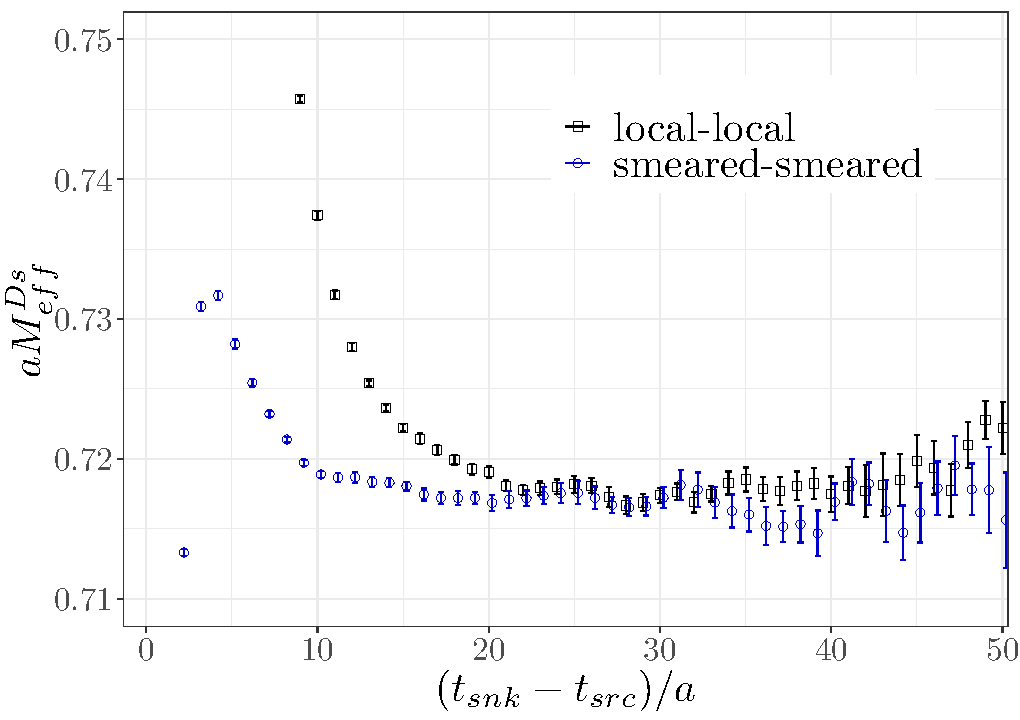
\includegraphics[width=0.59\textwidth]{plots/smearing_MDs.pdf}
  \caption{Comparison of the effective mass \eqref{eq:meff} of the correlator
    \eqref{eq:2pt}  computed with
    smeared quark field (smeared-smeared) and unsmeared (local-local)} 
  \label{fig:smearing}
\end{SCfigure}

For the contraction of the quark loops we will use nissa software
suite\footnote{nissa is public available at
\url{https://github.com/sunpho84/nissa}}, a C++  software for lattice
QCD calculations. The package provides the functionality for memory
distributed and shared memory systems and it supports all contractions 
needed for this proposal.

\subsection{The multi-grid solver}
The algorithms and codes to be used for this project are developed  for the NVIDIA GPU architecture
and thus are very well suited for the JUWELS booster module. For the solver we will use the QUDA library~\cite{Clark:2009wm,Babich:2011np,Clark:2016rdz} which provides optimised kernels for NVIDIA GPUs.
Simulations close to or at the physical point, like in this project, are  expensive, with the most computationally demanding component being the generation of quark propagators that require to invert the Dirac operator.

We will employ the state-of-the-art QUDA multigrid (MG) solver, a MG-preconditioned generalised conjugate residual (GCR) which has been further improved through the introduction of coarse-grid deflation.
Because we will employ twisted boundary conditions~\cite{deDivitiis:2004kq} to access arbitrary momentum configurations, we need to rerun the MG setup once for each phase angle.
As a result we will not make use of the coarse-grid deflated variant of the solver since the setup cost would then exceed the cost of the inversions for this particular project.
Still, the resulting solver is in a single solve much faster than the highly optimised implementation of the mixed-precision conjugate gradient (CG) algorithm in QUDA.
This is illustrated in \Cref{fig:multi-grid}, where we compare the time to solution between MG and mixed-precision CG for a range of valence quark masses ranging from the charm quark mass to the physical light quark mass.
The results obtained on a $64^3 \cdot 128$ lattice on eight JUWELS Booster nodes indicate that at the physical light quark mass, MG is more than 200 times faster than CG.
The disadvantage of MG solvers, however, is that they strong scale poorly due to the significantly smaller coarse grid system.

\begin{SCfigure}[0.5]
	\includegraphics[width=0.59\textwidth]{./plots/mg_vs_cg.pdf}
	\caption{Comparison between the time to solution for inverting the
    twisted mass clover Dirac matrix for one right-hand-side using
    the fastest mixed-precision CG in QUDA at different quark masses 
    against a tuned MG-preconditioned GCR on a $64^3\cdot128$ lattice
    on 8 nodes on JUWELS Booster. The dashed vertical lines indicate the
    approximate physical light ($\mu_{u,d}$), strange ($\mu_s$) and
    charm ($\mu_c$) quark masses.}
	\label{fig:multi-grid}
\end{SCfigure}

%% \textbf{Method}
%% \begin{itemize}
%%   \item depends on walltime, time-to-solution, time for contractions (plegma, quda )
%%     %%%
%%   \item low-mode deflation + hierarchical probing with 3 random vectors
%%     %%%
%%   \item volume sources ($\mathcal{O}(1000)$)
%%     %%%
%%   \item spin, color, time dilution ?
%%     %%%
%%   \item ``Frequency-splitting estimators of single-propagator traces'' ?
%%     %%%
%%   \item strange / charm loops ? OS / unitary ?
%% \end{itemize}

%\textbf{Misc}
%\begin{itemize}
%  \item meson-meson / baryon-baryon 2pt functions to build disc. contributions to ffs ? \\
%    \textbf{In case of renewal application:} do we have enough connected parts to demonstrate physics results / impa%ct of disc ?
%    %%%
%  \item smearing
%\end{itemize}


\endinput
